\documentclass[titlepage]{article}
\usepackage{graphicx}
\usepackage{wrapfig}
\usepackage{geometry}
\geometry{
 a4paper,
 total={170mm,257mm},
 left=20mm,
 top=20mm,
}

\usepackage{fancyhdr}
\fancypagestyle{pdf}{ 
    \fancyhf{} % clear all header and footer fields
    \fancyhead[L]{Practical Internet of Things with Raspberry Pi}
    \fancyhead[R]{Weather Station (WeatherDragon)}
    \fancyfoot[C]{\thepage}
    \setlength{\headheight}{13pt}
}
\pagestyle{pdf}

\title{Practical Internet of Things with Raspberry Pi\\ Project: Weather Station (WeatherDragon)}
\author{Marius-Catalin Ghiuri\\Leonard Hörnlein}
\date{\today}

\begin{document}
\maketitle
\newpage
\tableofcontents


\newpage
\section{Introduction}
\begin{wrapfigure}{r}{0.4\textwidth}
    \centering
    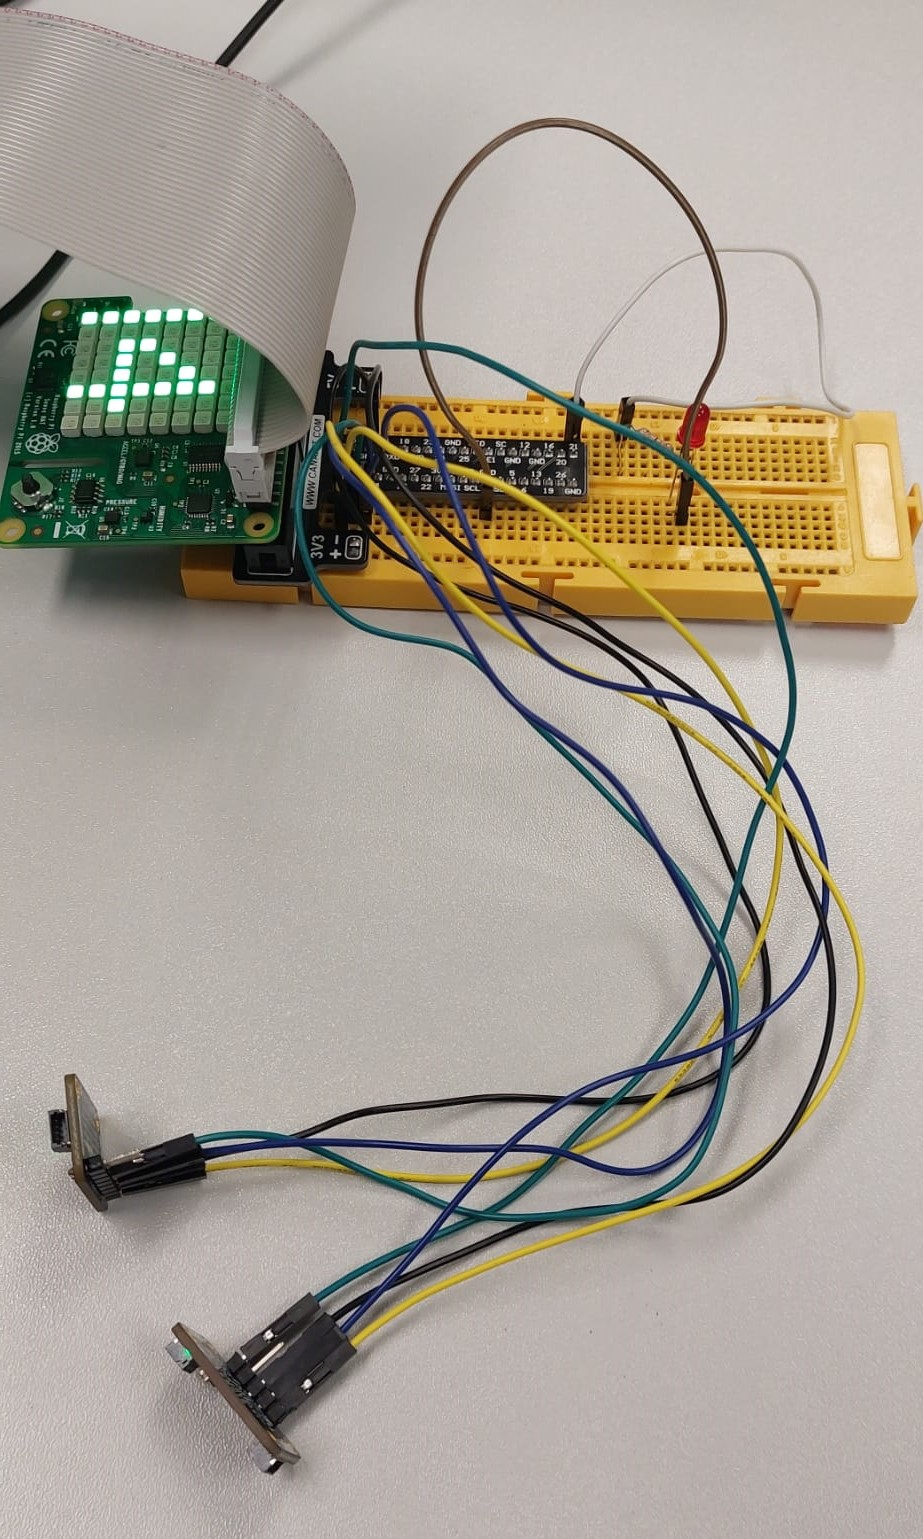
\includegraphics[width=0.3\textwidth]{img/dragon.jpg}
    \caption{Hardware setup}
    \label{fig:dragon}
\end{wrapfigure}

The project entails the construction of a comprehensive weather station. 
This station is equipped with sensors to measure temperature, humidity, and air pressure.\\
The Sense HAT's LED screen displays one of the three data parameters, selectable via a joystick.
Additionally, the text color on the LED screen dynamically changes based on predefined thresholds, with blue or red indicating values below or above acceptable limits, respectively, and green denoting normal conditions. 
In cases where at least one parameter exceeds the defined threshold for high values, a signal is visually conveyed through the blinking of an LED on the breadboard.\\
To monitor and analyze the data systematically, the project integrates with ThingSpeak, facilitating data uploads and providing a platform for visualization.\\
Furthermore, the system employs MQTT to enable remote monitoring via an app. 
In the event of sensed values surpassing predefined thresholds, an alarm is triggered, notifying the user through the app.


\newpage
\section{Hardware}
\begin{figure}[ht]
    \begin{minipage}{0.65\textwidth}
        The project runs on a Raspberry Pi 400, utilizing the Sense HAT as the central hardware component. 
        The Sense HAT serves as the primary interface for the weather station, providing essential functionalities for data display and interaction.\\
        In terms of sensors, the project incorporates two external sensors for more accurate readings. 
        The first is the Si7021 (Figure \ref{fig:Si7021}), dedicated to capturing temperature and relative humidity. 
        The second is the BMP390 (Figure \ref{fig:BMP390}), designed to measure temperature and air pressure.\\
        The decision to use external sensors, particularly for temperature, was motivated by the potential heat interference from the surrounding technology affecting the accuracy of the Sense HAT's onboard temperature sensor.
        Both external sensors are sourced from Adafruit, ensuring high-quality and reliable data acquisition.\\
        Additionally, an LED with an accompanying resistor is connected to the setup on the breadboard, serving as a visual indicator for specific threshold conditions, which are explained further on.\\
        The integration of these components on the breadboard forms the core infrastructure of the weather station system, providing a robust foundation for accurate and comprehensive environmental data monitoring.
    \end{minipage}
    %\hfill
    \begin{minipage}{0.3\textwidth} 
        \centering
        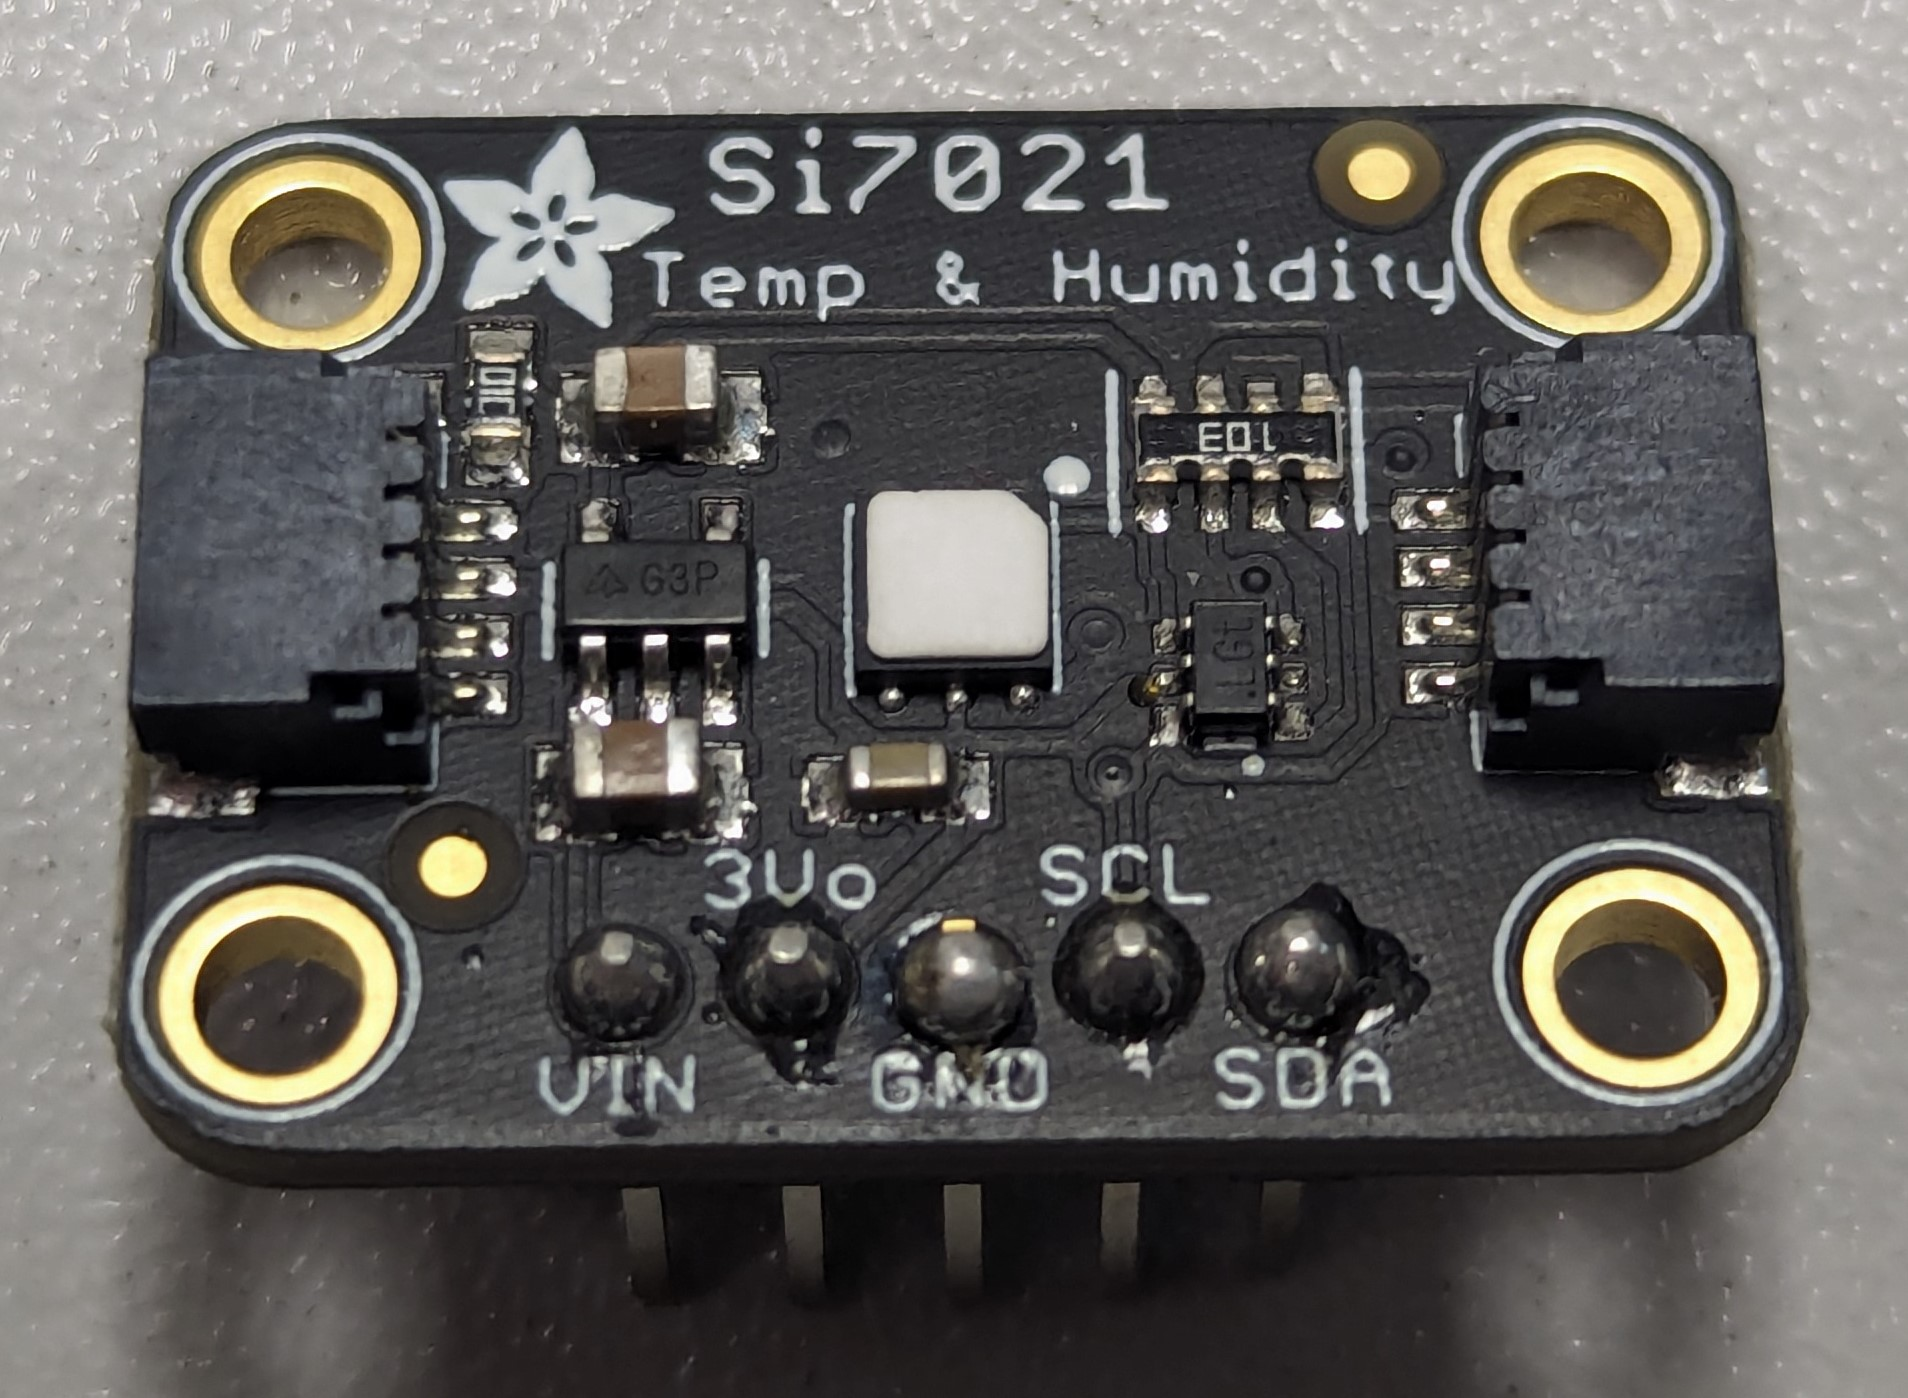
\includegraphics[width=0.6\textwidth]{img/Si7021.jpg}
        \caption{Si7021 sensor}
        \label{fig:Si7021}
        \vspace{1em}
        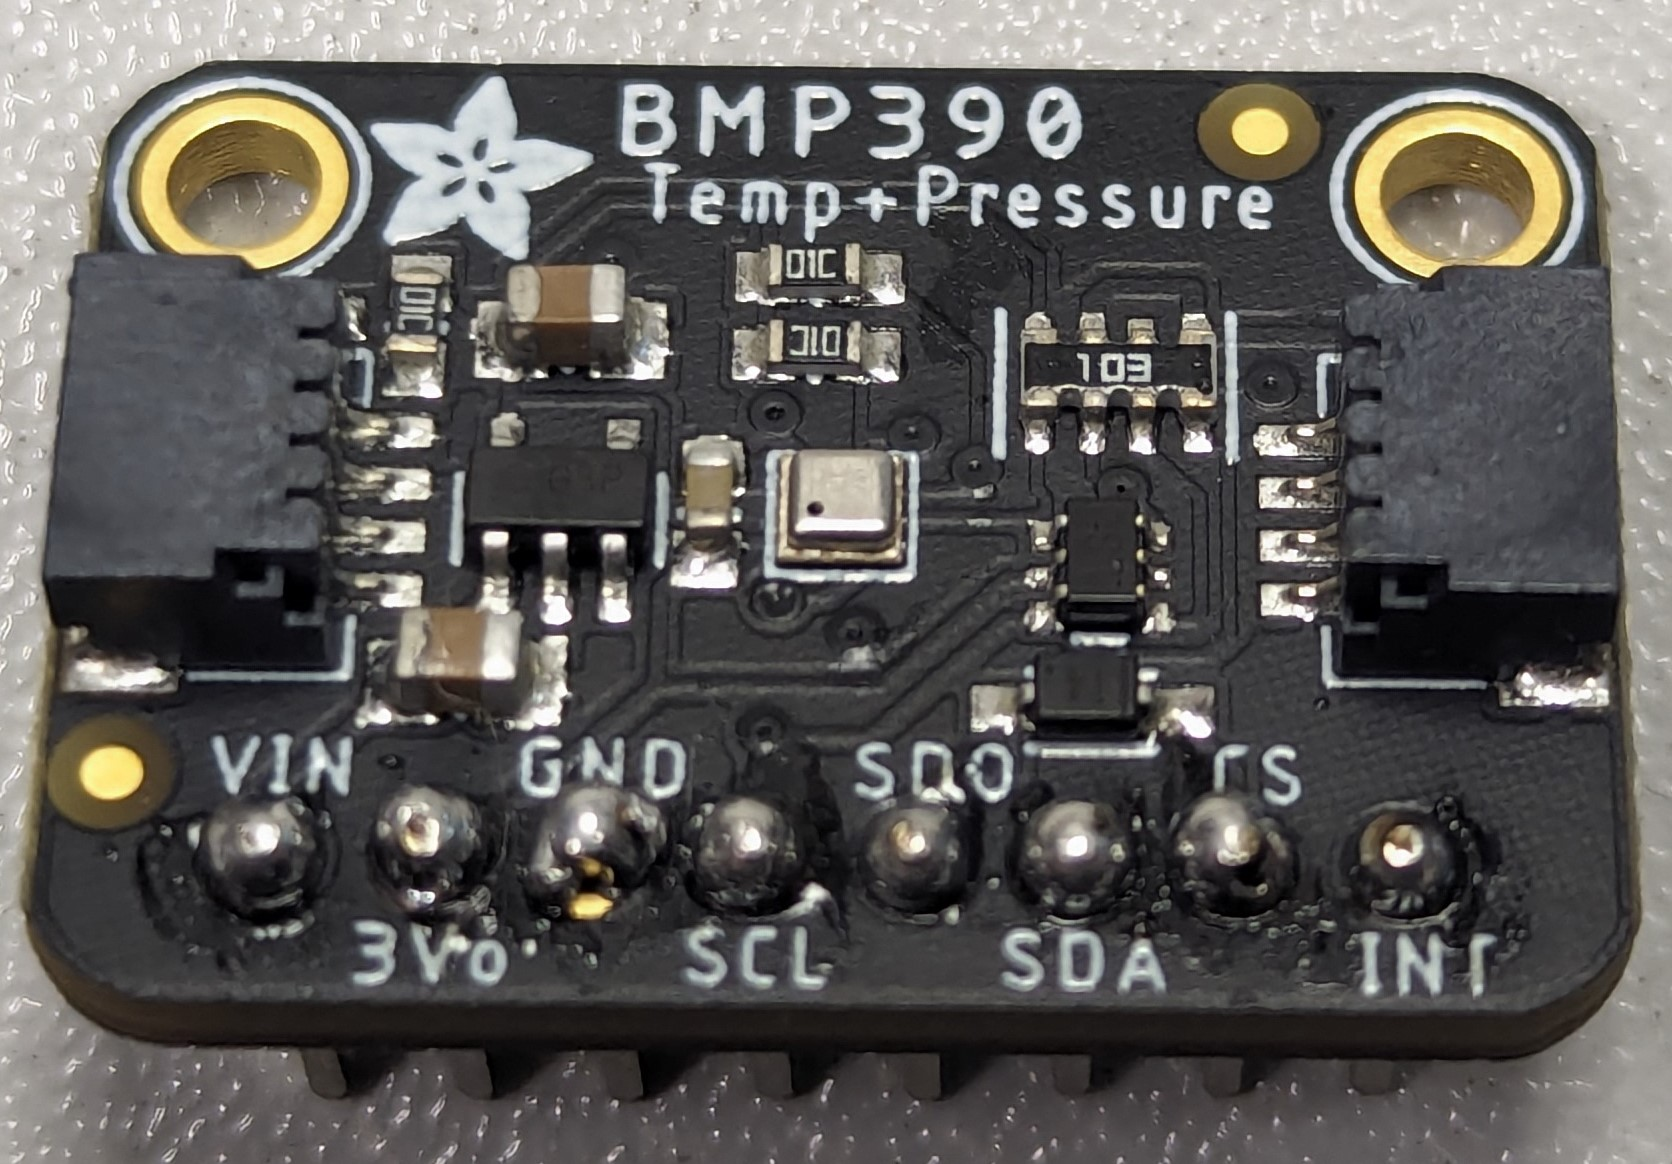
\includegraphics[width=0.6\textwidth]{img/BMP390.jpg}
        \caption{BMP390 sensor}
        \label{fig:BMP390}
    \end{minipage}
\end{figure}


\subsection{Hardware Connection}
In establishing the hardware connections, meticulous attention was given to ensure a robust and reliable configuration.\\
For both sensors, the grounding (\texttt{GND}) was seamlessly linked to a corresponding \texttt{GND} on the Raspberry Pi. 
The Serial Clock Line (\texttt{SCL}) and Serial Data Line (\texttt{SDA}) from each sensor found their designated counterparts on the Raspberry Pi, with both sensors sharing the same connection for streamlined communication. 
Furthermore, the \texttt{3Vo} (3.3V) outputs of the sensors were adeptly united with the \texttt{3Vo} on the Raspberry Pi, ensuring a consistent and stable power supply.\\
Concurrently, the LED was grounded to a \texttt{GND} pin on the Raspberry Pi, establishing a solid electrical reference. 
Its operational connection, intricately crafted, involved linking to \texttt{Pin 21}, ensuring precise control and integration with the broader system.\\
This meticulous arrangement, meticulously executed, forms the backbone of the hardware connections, guaranteeing optimal functionality and data integrity.

\begin{figure}[ht]
    \centering
    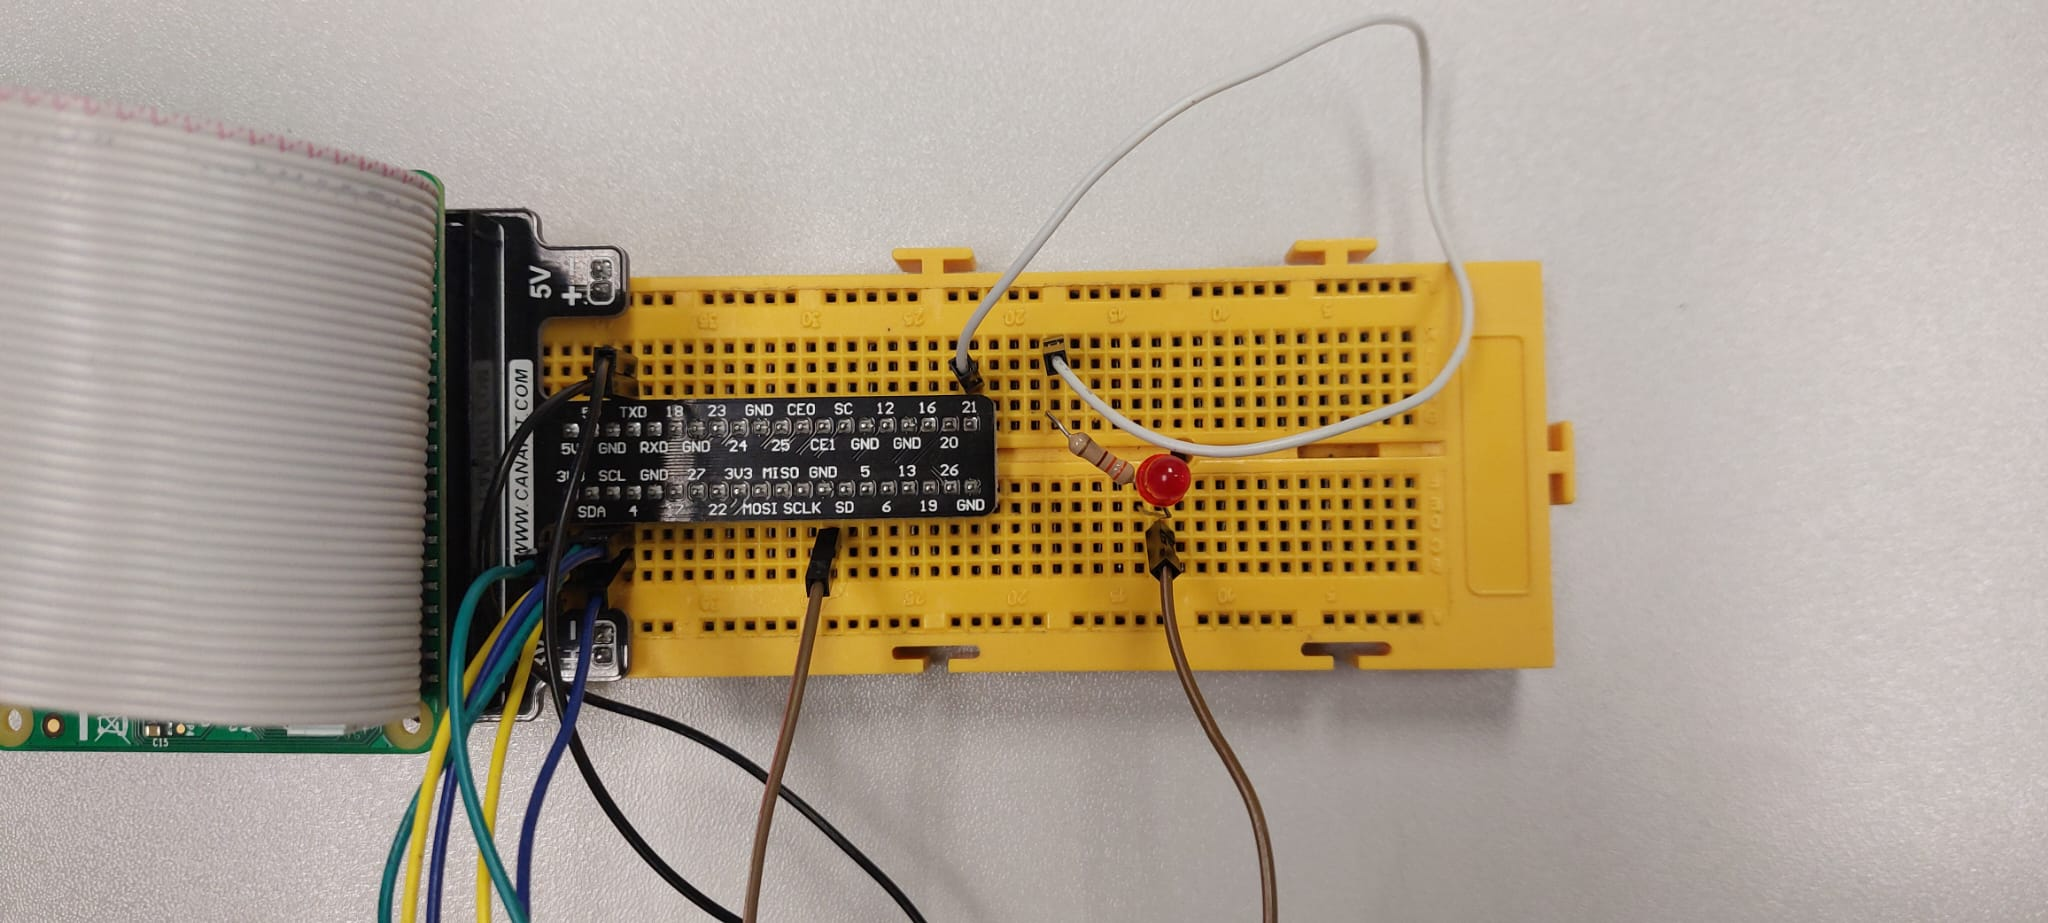
\includegraphics[width=0.5\textwidth]{img/cabels.jpg}
    \caption{Hardware Connections}
    \label{fig:cabels}
\end{figure}


\newpage

\section{Software Implementation}

The software implementation of the weather station project involves integrating various sensors, controlling the Sense HAT LED display, and communicating with external services for data storage and remote monitoring. The code is written in Python and takes advantage of libraries for sensor communication and data transmission.

\subsection{General Configuration}

The project uses several constants to define color thresholds and sensor limits. These include colors for the LED display (RED, GREEN, BLUE), minimum and maximum values for temperature (minTemp, maxTemp), humidity (minHum, maxHum), and pressure (minPrss, maxPrss).

\begin{verbatim}
# General Configuration
level = 0

RED = (255, 0, 0)
GREEN = (0, 255, 0)
BLUE = (0, 0, 255)

minTemp = 15
maxTemp = 30
minHum = 30
maxHum = 60
minPrss = 900
maxPrss = 1000
\end{verbatim}

\subsection{LED Control and Functions}

The code initializes the GPIO pin for the LED and defines functions for turning the LED on (\texttt{ledOn}), off (\texttt{ledOff}), and blinking (\texttt{ledBlink}). These functions are utilized later in the script to provide visual indications based on sensor readings.

\begin{verbatim}
# LED Control and Functions
LED_PIN = 21
GPIO.setmode(GPIO.BCM)
GPIO.setup(LED_PIN, GPIO.OUT)

def ledOn():
    GPIO.output(LED_PIN, GPIO.HIGH)

def ledOff():
    GPIO.output(LED_PIN, GPIO.LOW)

def ledBlink():
    ledOn()
    sleep(0.1)
    ledOff()
\end{verbatim}

\subsection{Sensor Configuration}

The code initializes and configures two sensors: the Si7021 for temperature and humidity, and the BMP3XX for temperature and pressure. The Adafruit CircuitPython libraries for each sensor are utilized for communication.

\begin{verbatim}
# Sensor Configuration
si = adafruit_si7021.SI7021(board.I2C())
bmp = adafruit_bmp3xx.BMP3XX_I2C(board.I2C())
\end{verbatim}

\newpage
\subsection{ThingSpeak Configuration}

The script defines parameters for ThingSpeak integration, including the ThingSpeak API key (\texttt{key}) and headers for data transmission. It also creates an HTTP connection to the ThingSpeak server.

\begin{verbatim}
# ThingSpeak Configuration
key = "<API KEY>"
headers = {"Content-type": "application/x-www-form-urlencoded"}
conn = http.client.HTTPConnection("api.thingspeak.com:80")
\end{verbatim}

\subsection{MQTT Configuration}

MQTT (Message Queuing Telemetry Transport) is configured with the broker address, and the script creates an MQTT client for publishing temperature, humidity, and pressure data.

\begin{verbatim}
# MQTT Configuration
broker_address = "broker.emqx.io"
client = mqtt.Client()
client.connect(broker_address, 1883, 60)
client.loop_start()
\end{verbatim}

\subsection{Main Loop}

The main loop continuously reads sensor data, updates the LED display on the Sense HAT, uploads data to ThingSpeak, and publishes data to MQTT topics for remote monitoring.

\begin{verbatim}
# Main Loop
while True:
    # ... (Sensor readings, ThingSpeak upload, Sense HAT display, MQTT publishing)

\end{verbatim}


\subsubsection{Sensor Data Reading}
Sensor data, including temperature (\texttt{temp}), humidity (\texttt{hum}), and pressure (\texttt{prss}), is continuously acquired from the Si7021 and BMP3XX sensors.
For the temperature, we calculate the mean of both sensors to get an better result.

\begin{verbatim}
temp = round((round(bmp.temperature, 1) + round(si.temperature, 1)) / 2, 1)
hum = round(si.relative_humidity, 1)
prss = round(bmp.pressure, 1)
\end{verbatim}

\subsubsection{ThingSpeak Data Upload}
The acquired sensor data is then uploaded to ThingSpeak using HTTP POST requests. The data, along with the ThingSpeak API key, is formatted and sent to the ThingSpeak server.

\begin{verbatim}
params = urllib.parse.urlencode({
    'field1': temp,
    'field2': hum,
    'field3': prss,
    'key': key
})

conn.request("POST", "/update", params, headers)
response = conn.getresponse()
\end{verbatim}

\newpage
\subsubsection{Sense HAT Display}
The Sense HAT LED display is updated based on the sensor readings. Color-coded messages are displayed to indicate the status of temperature, humidity, and pressure.

\begin{verbatim}
# Sense HAT Display
if hum > maxHum:
    hum_color = RED
    ledBlink()
elif hum > minHum:
    hum_color = GREEN
else:
    hum_color = BLUE

# ... (Similar logic for temperature and pressure)

# Sense HAT message display based on the selected data parameter
for event in sense.stick.get_events():
    if event.direction == "up" and event.action == "pressed":
        level = (level + 1) % 3
    # ... (Additional logic for joystick input and message display)
\end{verbatim}

\subsubsection{MQTT Publishing}
The acquired sensor data is published to MQTT topics for remote monitoring. Topics include "/temperature," "/humidity," and "/pressure."

\begin{verbatim}
# MQTT Publishing
client.publish("/temperature", temp)
client.publish("/humidity", hum)
client.publish("/pressure", prss)
\end{verbatim}


\newpage
\section{Results}

As a user, data visualization and monitoring options are provided through multiple channels:

\subsection{Sense HAT and Breadboard}
The Sense HAT display presents real-time environmental data, focusing on one of the three parameters (temperature, humidity, or pressure) at a time. Users can navigate between these parameters using the joystick (up and down). The text color on the display dynamically changes based on predefined thresholds: green signifies values within the normal range, blue indicates values below, and red indicates values above acceptable limits. In case a parameter exceeds the defined upper threshold, the LED blinks as a warning.

\subsection{IoT MQTT Panel App}
For a convenient and real-time overview of the current weather conditions, users can utilize the IoT MQTT Panel app (see Figure \ref{fig:app-iot}). The app displays the latest temperature, humidity, and pressure values, providing a mobile interface for on-the-go monitoring.

\subsection{MQTT Alert App}
The MQTT Alert app (see Figure \ref{fig:app-alert}) offers customization for threshold-based alerts. Users can set alarms to trigger when sensor values surpass predefined limits. This feature enhances proactive monitoring, allowing users to receive immediate notifications on their mobile devices in case of unfavorable environmental conditions.


\begin{figure}[ht]
    \begin{minipage}{0.48\textwidth}
        \centering
        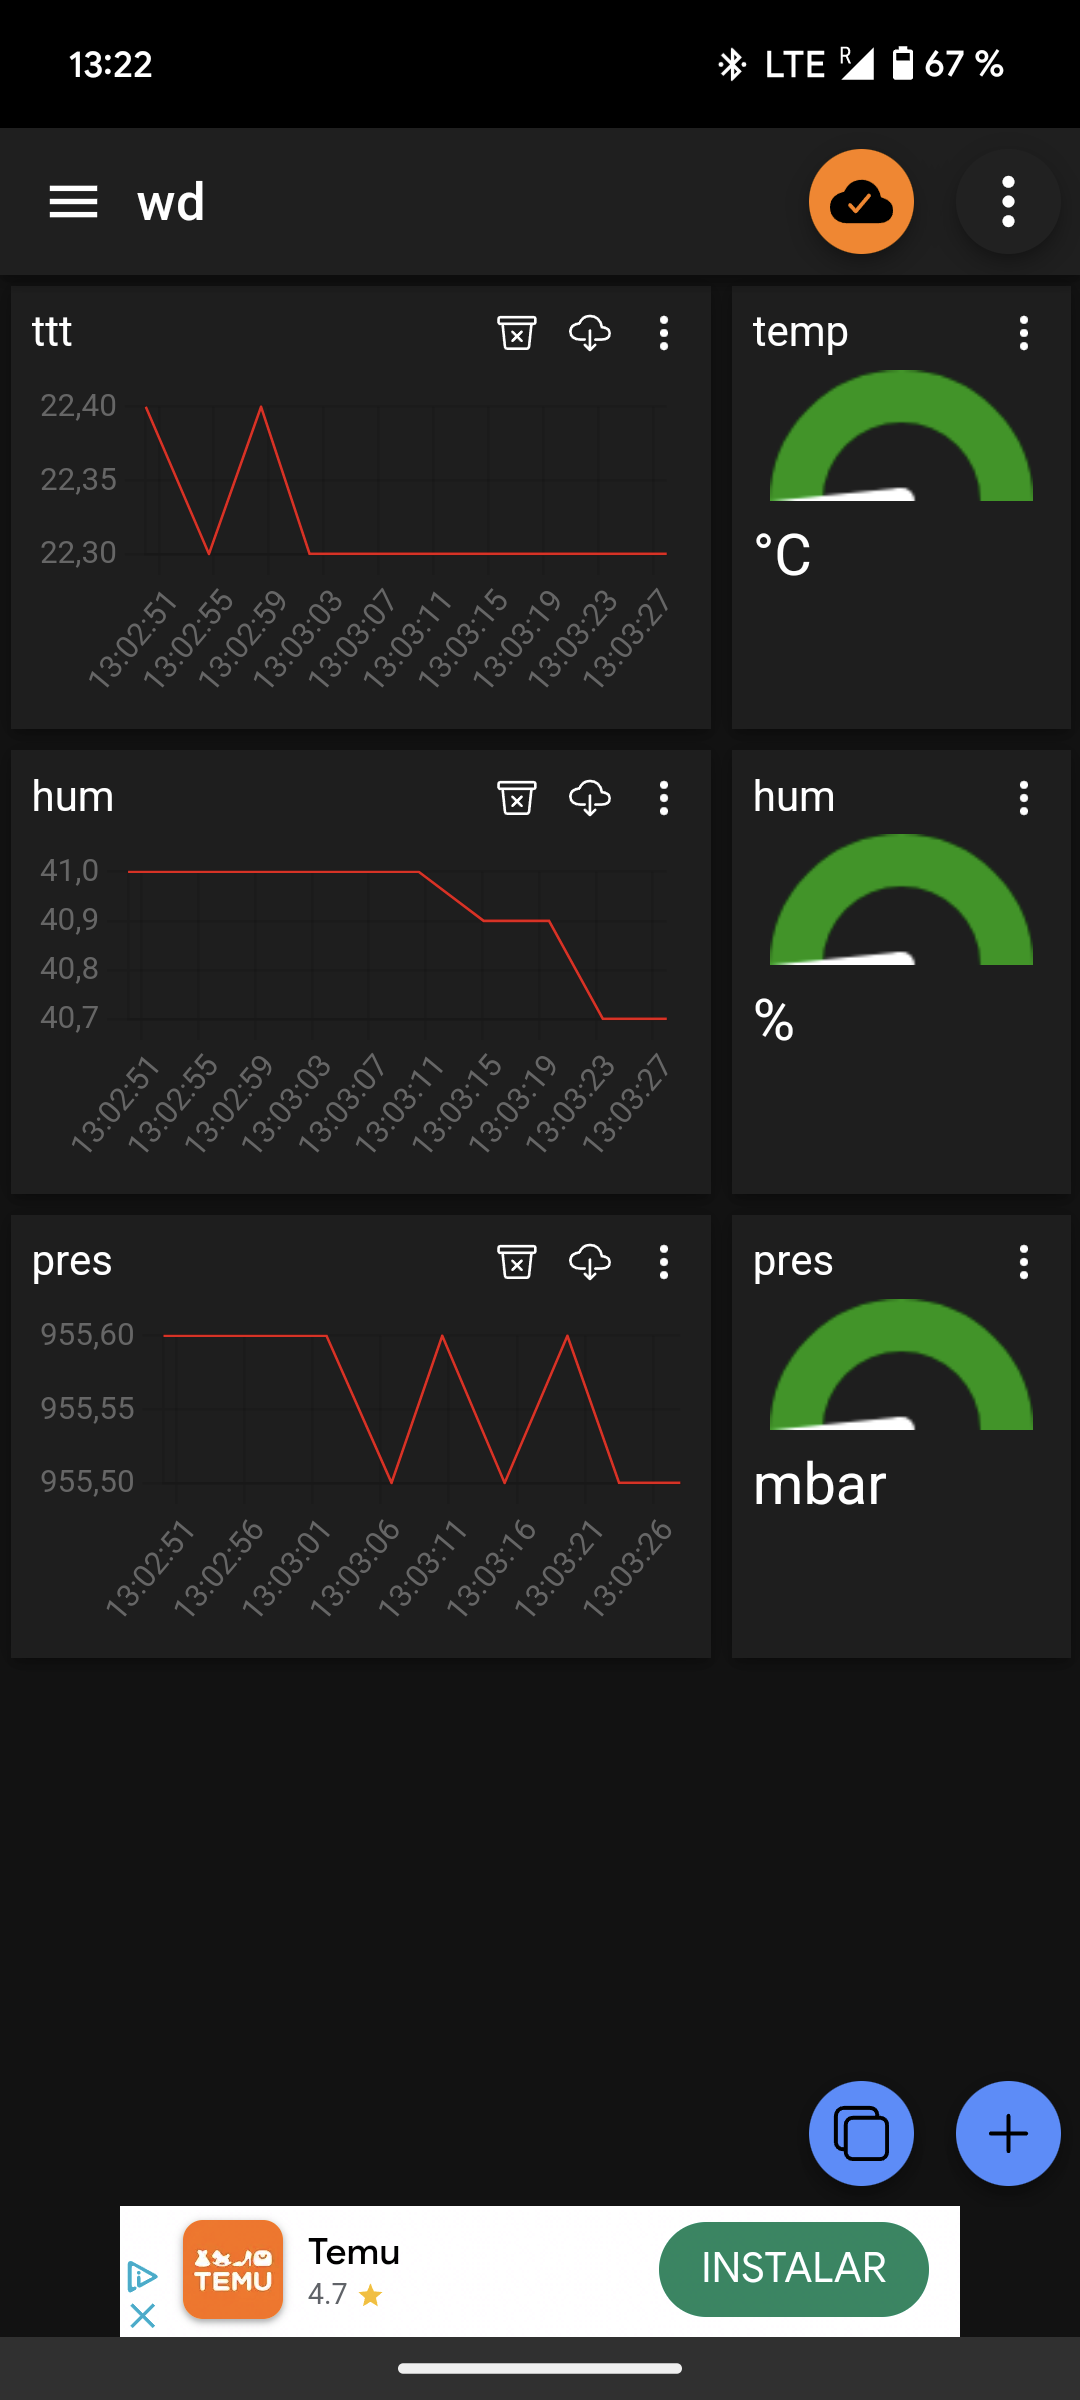
\includegraphics[width=0.5\textwidth]{img/App-IoT.png}
        \caption{IoT MQTT Panel App}
        \label{fig:app-iot}
    \end{minipage}
    \hfill
    \begin{minipage}{0.48\textwidth}
        \centering
        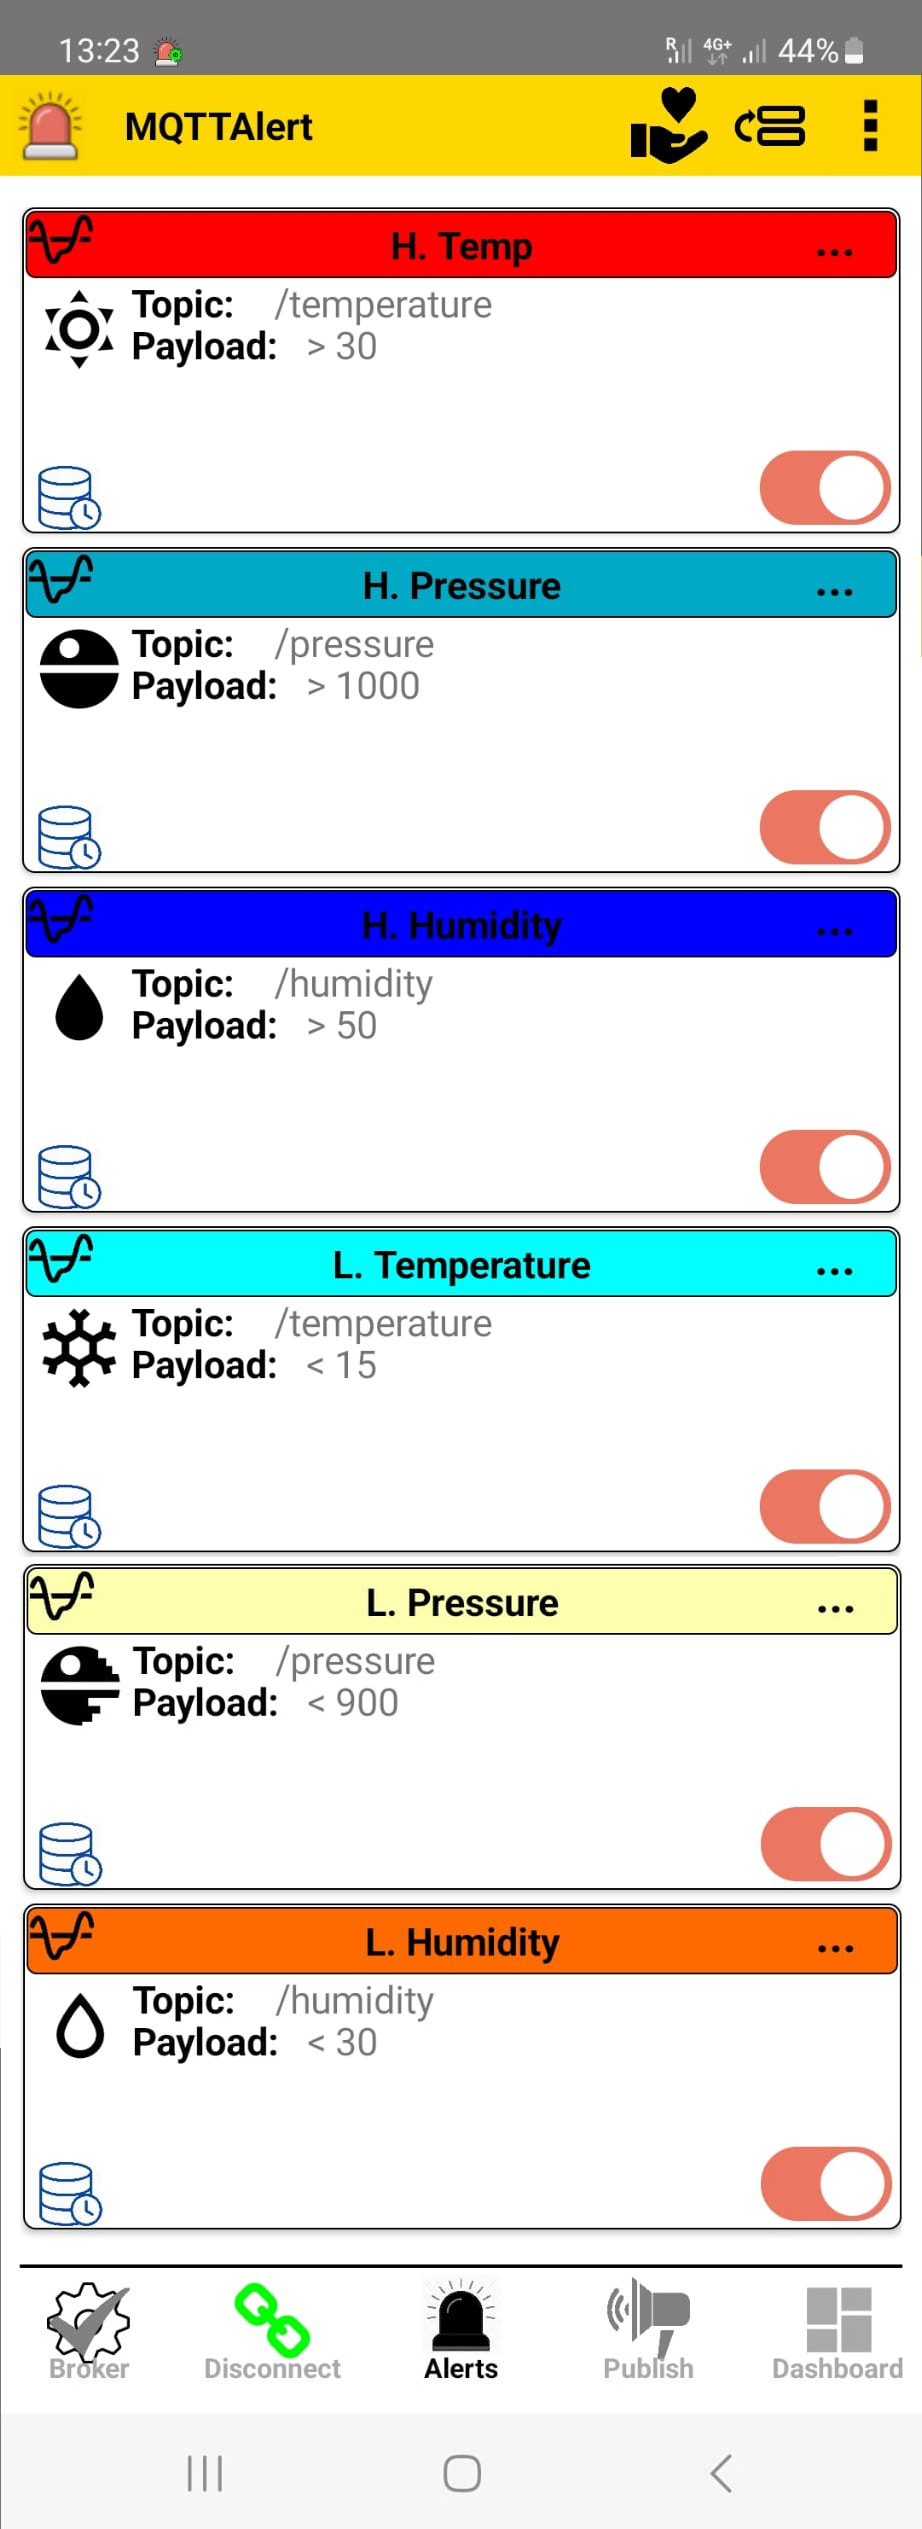
\includegraphics[width=0.5\textwidth]{img/App-Alert.jpg}
        \caption{MQTT Alert App}
        \label{fig:app-alert}
    \end{minipage}
\end{figure}

\newpage
\subsection{ThingSpeak Online Platform}
For long-term data tracking and analysis, users can access the ThingSpeak online platform (see Figure \ref{fig:thingspeak}). ThingSpeak provides a comprehensive view of historical data, enabling users to observe trends and patterns over time.


\begin{figure}[ht]
    \centering
    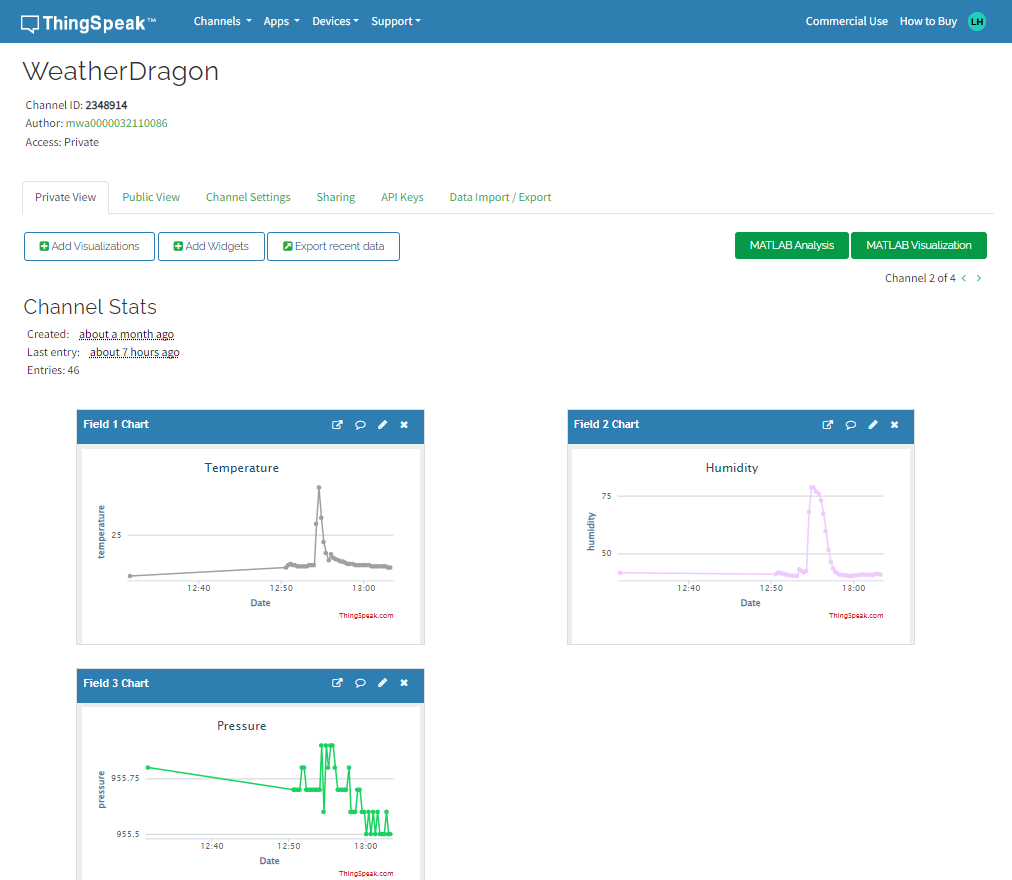
\includegraphics[width=0.6\textwidth]{img/thingspeak.png}
    \caption{ThingSpeak Online Platform}
    \label{fig:thingspeak}
\end{figure}



\end{document}